% ===== 原文 pp.38--42（tr-03 第 1 段；接 tr-02 的 (4.18) 及其在本页顶部写完的那一段之后）=====
% [原文 p.38]

只要不只调节 $u$，我们就能让两个以上的分支点同时碰撞，从而让不止一组场变得无质量。这类极限在红外可以导致非平凡的 SCFT，其中包括 AD 理论------我们会在第 7 节回到它。这些极限在二维一侧也同样有意思。

\para{耦合常数。} $q=\ee^{2\pi\ii\tau}$ 取值遍历 $\C\setminus\{0,1\}$，它究竟如何重现带 $N_f=4$ 的 $\mathrm{SU}(2)$ SQCD 拉氏量描述中出现的那一个复化规范耦合 $\tau_{\mathrm{Lag}}=\theta/(2\pi)+4\pi\ii/g^2$------尤其是 $\Im\tau_{\mathrm{Lag}}>0$ 这一点------初看颇令人困惑。为了把二者联系起来，我们考虑所有 $m_i\to0$ 的无质量极限：此时理论是一个 SCFT，耦合不跑动。等价的极限是 Coulomb 分支上 $|u|$ 很大的区域，具体说是 $|u|\gg|m_i|^2$。从这个角度看，重整化群的跑动在很大的能标 $|u|$ 处就很快停止了。于是，SW 曲线所捕捉到的红外规范耦合 $\tau_{\mathrm{IR}}$ 满足 $\tau_{\mathrm{IR}}=2\tau_{\mathrm{Lag}}$；那个因子源自 $\mathrm{U}(1)$ 嵌入 $\mathrm{SU}(2)$ 的方式。

SW 曲线 $\Sigma$ 是一个双覆盖球面的环面，它的四个分支点位于 $u_2$ 的零点处。式 (4.13) 给出的 $u_2$ 中前四项里，同一时刻至多只有一项可以很大，因此为了抵消 $u$ 的大值，$z$ 必须靠近穿刺点 $0,q,1,\infty$ 之一：于是四个分支点分别位于
\begin{equation}
  z=O\!\left(\frac{m_1^2}{u}\right),\qquad
  z=q+O\!\left(\frac{m_2^2}{u}\right),\qquad
  z=1+O\!\left(\frac{m_3^2}{u}\right),\qquad
  z=O\!\left(\frac{u}{m_4^2}\right).
  \tag{4.19}
\end{equation}

% [Tutor Note: p.38 式 (4.19) 的量纲自查：前三式给出 $z-z_i=O(m_i^2/u)$；第四个穿刺点在 $z=\infty$，换到局部坐标 $w=1/z$ 后同一论证给出 $w=O(m_4^2/u)$，即 $z=O(u/m_4^2)$。"偏离距离 × 斜率" 四式互为倒数，可用来核对是否把分子分母抄反。]

环面 $\Sigma$ 的模参数 $\tau_{\mathrm{IR}}$ 给出复化规范耦合，它自动满足 $\Im\tau_{\mathrm{IR}}>0$。用模 lambda 函数 $\lambda$ 表示，有 [177]
\begin{equation}
\begin{aligned}
  q &= \lambda(\tau_{\mathrm{IR}})=16\,\ee^{\pi\ii\tau_{\mathrm{IR}}}
       -128\,\ee^{2\pi\ii\tau_{\mathrm{IR}}}+\dots,\\
  \tau &= \half\tau_{\mathrm{IR}}+\frac{\log 16}{2\pi\ii}
       -\frac{8}{2\pi\ii}\,\ee^{\pi\ii\tau_{\mathrm{IR}}}+\dots,
\end{aligned}
  \tag{4.20}
\end{equation}
这里的展开适用于小规范耦合 $g$。$\tau$ 与 $\tau_{\mathrm{Lag}}=\half\tau_{\mathrm{IR}}$ 都是完全合格的规范耦合定义，二者只相差两种不同的重整化方案：差一个常数平移，外加瞬子修正。重新定义耦合的自由度在式 (5.38) 处还会再次出现。

% [Tutor Note: p.38 式 (4.20) 可用标准椭圆模函数核对：$\lambda(\tau)=16q-128q^2+704q^3-\dots$（此处 $q=\ee^{\pi\ii\tau}$）。原文前两个系数 $16$、$-128$ 与标准值一致；需要时可用第三项 $704$ 区分 $q=\ee^{\pi\ii\tau}$ 与 $q=\ee^{2\pi\ii\tau}$ 两种约定。第二式亦可反解验证：由 $\tau=\frac{1}{2\pi\ii}\log(q/16)+O(q)$ 可知，常数项 $\log16/(2\pi\ii)$ 正是把 $\ee^{2\pi\ii\tau}$ 归一成 $q$ 的那个平移。]

\para{S 对偶。} 四穿刺球面 $\mathbb{CP}^1\setminus\{0,q,1,\infty\}$ 有三种裤子分解，因而有三种拉氏量描述。这些描述除了质量的置换 $m_1,m_2,m_3,m_4$ 以及把 $q\to1/q$ 或 $q\to1-q$ 之外完全相同。这就是 SQCD 的 S 对偶 [4]。按式 (4.11) 的记号，
\begin{equation}
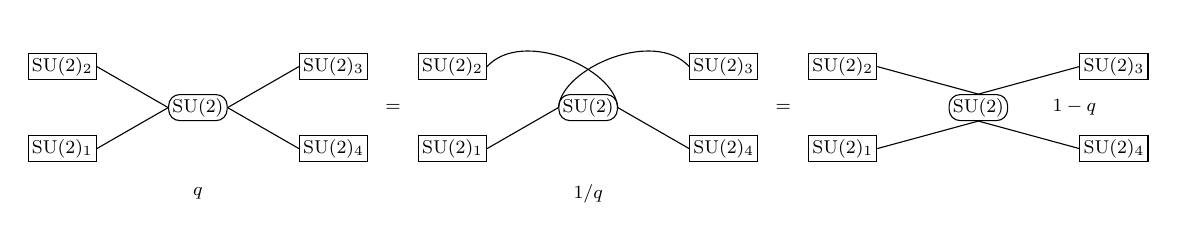
\begin{tikzpicture}[baseline=(G.center),scale=0.84,transform shape,
  fl/.style={draw,rectangle,inner sep=1.6pt,font=\footnotesize},
  ga/.style={draw,rounded corners=4pt,inner sep=1.6pt,font=\footnotesize}]
  % ---- 第一张图：耦合 q ----
  \node[ga] (G) at (0,0) {$\mathrm{SU}(2)$};
  \node[fl] (Lt) at (-2.05,0.62) {$\mathrm{SU}(2)_2$};
  \node[fl] (Lb) at (-2.05,-0.62){$\mathrm{SU}(2)_1$};
  \node[fl] (Rt) at (2.05,0.62) {$\mathrm{SU}(2)_3$};
  \node[fl] (Rb) at (2.05,-0.62){$\mathrm{SU}(2)_4$};
  \draw (Lt.east) -- (G.west);
  \draw (Lb.east) -- (G.west);
  \draw (G.east) -- (Rt.west);
  \draw (G.east) -- (Rb.west);
  \node[font=\footnotesize] at (0,-1.3) {$q$};
  % ---- 等号 ----
  \node[font=\footnotesize] at (2.95,0) {$=$};
  % ---- 第二张图：耦合 1/q（两条连线交叉）----
  \node[ga] (G2) at (5.9,0) {$\mathrm{SU}(2)$};
  \node[fl] (Lt2) at (3.85,0.62) {$\mathrm{SU}(2)_2$};
  \node[fl] (Lb2) at (3.85,-0.62){$\mathrm{SU}(2)_1$};
  \node[fl] (Rt2) at (7.95,0.62) {$\mathrm{SU}(2)_3$};
  \node[fl] (Rb2) at (7.95,-0.62){$\mathrm{SU}(2)_4$};
  \draw (Lt2.east) .. controls (4.9,1.2) and (6.3,0.6) .. (G2.east);
  \draw (Rt2.west) .. controls (6.9,1.2) and (5.5,0.6) .. (G2.west);
  \draw (Lb2.east) -- (G2.west);
  \draw (Rb2.west) -- (G2.east);
  \node[font=\footnotesize] at (5.9,-1.3) {$1/q$};
  % ---- 等号 ----
  \node[font=\footnotesize] at (8.85,0) {$=$};
  % ---- 第三张图：耦合 1-q ----
  \node[ga] (G3) at (11.8,0) {$\mathrm{SU}(2)$};
  \node[fl] (Lt3) at (9.75,0.62) {$\mathrm{SU}(2)_2$};
  \node[fl] (Lb3) at (9.75,-0.62){$\mathrm{SU}(2)_1$};
  \node[fl] (Rt3) at (13.85,0.62) {$\mathrm{SU}(2)_3$};
  \node[fl] (Rb3) at (13.85,-0.62){$\mathrm{SU}(2)_4$};
  \draw (Lt3.east) -- (G3.north);
  \draw (Rt3.west) -- (G3.north);
  \draw (Lb3.east) -- (G3.south);
  \draw (Rb3.west) -- (G3.south);
  \node[font=\footnotesize,anchor=west] at (12.8,0) {$1-q$};
\end{tikzpicture}
  \tag{4.21}
\end{equation}

这些等式在 6d 视角下是显然的，但它们背后藏着深刻的非微扰物理：它们所联系的是若干涉及完全不同的基本规范场与物质场的量子场论（某个描述里的规范场 $A_\mu$ 与另一个描述里的 $A_\mu$ 并无关系）。

% [Tutor Note: p.39 式 (4.21) 的三张图是同一 4d 理论的三种 S 对偶描述：(左) 直连，(中) 两条双基本表示连线交叉，(右) 端点改接到节点上下两端。判读要点是"哪个味 $\mathrm{SU}(2)$ 接到规范节点的哪一侧"------中间那张把上下两组味因子的角色对调，正是 $q\to1/q$ 的体现；这也解释了习题 4.10 第 2 问：对不同规范节点施加基本 S 对偶彼此不对易。]

% [原文 p.39]

\subsection{广义 $\mathrm{SU}(2)$ 箭图}

我们已经给出了所需的全部材料，用来确定 $\cX(\fsu(2))$ 在任意带驯服穿刺点的穿刺黎曼面 $C$ 上给出的 $\fsu(2)$ class S 理论。\footnote{我们排除没有穿刺点的球面、一个穿刺点（平面）或两个穿刺点（圆柱）的情形，以及没有穿刺点的环面，因为它们都是病态的。}因此本小节基本上就是一堆习题。

\para{五穿刺球面。} 这里取 $C=\mathbb{CP}^1\setminus\{0,z_1,z_2,1,\infty\}$；注意与先前约定相比，我们把穿刺点 $z_i$ 的编号平移了一点。对任意一种分解成三穿刺球面的方式，拉氏量都具有如下形式
\begin{equation}
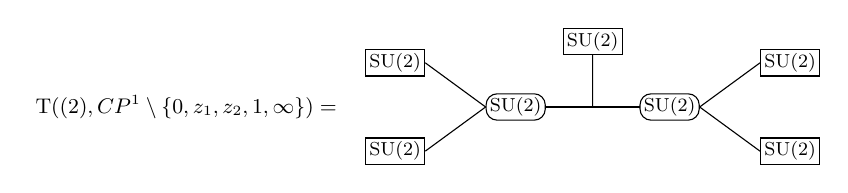
\begin{tikzpicture}[baseline=(G1.center),scale=0.85,transform shape,
  fl/.style={draw,rectangle,inner sep=1.6pt,font=\footnotesize},
  ga/.style={draw,rounded corners=4pt,inner sep=1.6pt,font=\footnotesize}]
  \node[font=\small,anchor=east] at (-1.35,0) {$\mathrm{T}(\fsu(2),\mathbb{CP}^1\setminus\{0,z_1,z_2,1,\infty\})=$};
  \node[ga] (G1) at (1.2,0) {$\mathrm{SU}(2)$};
  \node[ga] (G2) at (3.5,0) {$\mathrm{SU}(2)$};
  \node[fl] (A) at (-0.6,0.66) {$\mathrm{SU}(2)$};
  \node[fl] (B) at (-0.6,-0.66){$\mathrm{SU}(2)$};
  \node[fl] (M) at (2.35,0.98) {$\mathrm{SU}(2)$};
  \node[fl] (D) at (5.3,0.66) {$\mathrm{SU}(2)$};
  \node[fl] (E) at (5.3,-0.66){$\mathrm{SU}(2)$};
  \draw (A.east) -- (G1.west);
  \draw (B.east) -- (G1.west);
  \draw (G1.east) -- (G2.west);
  \draw (M.south) -- (2.35,0);
  \draw (G2.east) -- (D.west);
  \draw (G2.east) -- (E.west);
\end{tikzpicture}
  \tag{4.22}
\end{equation}

与穿刺点更少的球面不同，从 6d 明显可见的 $\mathrm{SU}(2)^5$ 味对称性在 4d 理论中不会增强（就我所知）。这个理论的 S 对偶在 class S 理论出现之前就已在 [175] 中研究过，而它们的 S 对偶是在 [1] 中被揭示的。

\begin{exercise}{4.8}
按习题 3.3 的做法，把 $C$ 写成三个裤子的粘合，粘合参数为 $z_1/z_2$ 与 $z_2$。
\end{exercise}

\begin{exercise}{4.9}
对 $C$ 的每一种裤子分解，验证其拉氏量描述就是 (4.22)：规范群为 $\mathrm{SU}(2)^2$，含十二个超多重态。它们按 $\mathrm{SU}(2)^2$ 规范群的什么表示变换？这些表示又带有哪些味对称性？
\end{exercise}

\begin{exercise}{4.10}
\begin{enumerate}[label=\arabic*.,leftmargin=2em,itemsep=1pt,topsep=1pt]
\item 每个 $\mathrm{SU}(2)$ 规范群都与四个双重态超多重态耦合。当另一个规范群弱耦合时，这个理论就是 SQCD 再通过一个弱耦合规范场与额外物质耦合。对这个 SQCD 理论“施加”S 对偶，验证所得描述正是你会为五穿刺球面的某个裤子写下的描述。
% [原文 p.40]
\item 验证把基本 S 对偶 (4.21) 施加到不同规范节点上并不对易，因此 $\mathrm{SU}(2)^2$ 规范理论的 S 对偶群（胚）不是两个 SQCD 理论 S 对偶群的乘积。
\end{enumerate}
\end{exercise}

\para{穿刺球面。} 接下来考虑带 $n$ 个穿刺点的 $\mathbb{CP}^1\setminus\{z_0,\dots,z_{n-1}\}$，其中 $z_0=0$、$z_{n-2}=1$、$z_{n-1}=\infty$。记 $m_0,m_1,\dots,m_{n-1}$ 为各穿刺点的质量参数。

\begin{exercise}{4.11}
\begin{enumerate}[label=\arabic*.,leftmargin=2em,itemsep=1pt,topsep=1pt]
\item 像习题 4.3 与习题 4.5 那样使用 Liouville 定理，求出所有在穿刺点处具有指定二阶极点的二次微分 $\phi_2(z)$。由此推出 Coulomb 分支为 $\cB=\C^{n-3}$。
\item 写出该理论的 $\mathrm{SU}(2)^{n-3}$ 线性箭图描述，它在 $|z_1|\ll|z_2|\ll\dots\ll|z_{n-3}|\ll1$ 的区域内弱耦合。
\item 在此区域内，对位于圆环 $|z_{i-1}|\ll|z|\ll|z_{i+1}|$（$i=1,\dots,n-2$）中的 $z$ 展开 $\phi_2(z)$。验证在每一块裤子构件上 $\phi_2$ 都化为 $T_2$ 的微分。验证 $\cB=\C^{n-3}$ 可以用这些裤子中穿刺点的参数 $u_i$（$i=1,\dots,n-3$）来参数化。并确认 $u_i=\half\Tr\phi_i^2$，其中 $\phi_i$ 是第 $i$ 个矢量多重态的标量。
\item 验证：从 $n=6$ 开始，裤子分解除了穿刺点的置换之外还可以在拓扑上不同。
\end{enumerate}
\end{exercise}

% [Tutor Note: 原文 p.40 习题 4.11 的小问编号有笔误：四个小问印作 1.、2.、2.、3.（第三问重复了 2.，末问错成 3.）。译文按内容排成 1.--4.，此处记录原文面貌以便对照。]

\para{穿刺环面。} 我们对亏格 $g=1$ 重复类似的练习。也可以研究与更高亏格曲线相联系的理论，但所需数学超出了本综述的范围。

\begin{exercise}{4.12}
\begin{enumerate}[label=\arabic*.,leftmargin=2em,itemsep=1pt,topsep=1pt]
\item 单穿刺环面是把同一个裤子的两个穿刺点粘合而得到的。把该理论写成 $\mathrm{SU}(2)$ 规范理论，并注意到除了伴随超多重态之外还存在一个解耦的规范单态。\footnote{在考虑 $n$ 穿刺环面或更高亏格曲面的不同拉氏量描述时，这类规范单态究竟如何成立，我目前还不很清楚。的确，有些通道包含伴随超多重态，因而包含规范单态；而在另一些通道里这些单态并不显然。}
\item 把与 $n$ 穿刺环面相联系的理论写成一个环形的 $\mathrm{SU}(2)^n$ 箭图：每一对相邻群之间有一个双基本表示超多重态。弱规范耦合区域对应于一个细长、穿刺点彼此远离的环面。
\item 如果你对椭圆函数足够熟悉，就定出所有在穿刺点处具有指定二阶极点的二次微分。像习题 4.11 那样把它们在弱规范耦合极限下展开。
\end{enumerate}
\end{exercise}

\subsection{线性箭图 $\fsu(N)$ 理论}

下面简要转向 $\fsu(N)$ class S 理论，特别是其中一个从 6d 角度看颇为 ad-hoc、但在 4d 会给出线性箭图规范理论的子类；这一点可以借助膜构造来理解。它们对我们后面讨论瞬子很有用。

% [原文 p.41]

\para{共形 SQCD。} 我们试着把带 $N_f=2N$ 个味（这是贝塔函数为零所需的味数）的 $\mathrm{SU}(N)$ SQCD 实现为 class S 理论。它的味对称性是 $\fu(N_f)=\fu(2N)$（当 $N=2$ 时增强为 $\fso(8)$）。类比 $N=2$ 的情形，我们预期规范群对应于连接两个三穿刺球面的管子，于是把 $2N$ 个味分成两组、每组 $N$ 个，而每组应当来自两个三穿刺球面之一。每组的味对称性是 $\fu(N)=\fu(1)\times\fsu(N)$，因此这种分法使 $\fsu(N)^2\times\fu(1)^2$ 味对称性成为显然。仿照 $N=2$ 的情形，我们把四个因子各联系到一个穿刺点，并写下 (4.11) 的类似物：\footnote{与本综述其他若干处一样，这里关于群的全局结构有不准确之处。欢迎指正。}
\begin{equation}
\begin{tikzpicture}[baseline=(G.center),scale=0.85,transform shape,
  fl/.style={draw,rectangle,inner sep=1.8pt,font=\footnotesize},
  ga/.style={draw,rounded corners=4pt,inner sep=1.8pt,font=\footnotesize}]
  \node[font=\small,anchor=east] at (-1.55,0) {$\mathrm{T}(\fsu(N),\mathbb{CP}^1\setminus\{4\text{ 点}\},\text{合适的数据})=$};
  \node[ga] (G) at (1.2,0) {$\mathrm{SU}(N)$};
  \node[fl] (UL) at (-0.75,0.62) {$\mathrm{U}(1)$};
  \node[fl] (SL) at (-0.75,-0.62){$\mathrm{SU}(N)$};
  \node[fl] (UR) at (3.15,0.62) {$\mathrm{U}(1)$};
  \node[fl] (SR) at (3.15,-0.62){$\mathrm{SU}(N)$};
  \draw (UL.east) -- (G.west);
  \draw (SL.east) -- (G.west);
  \draw (G.east) -- (UR.west);
  \draw (G.east) -- (SR.west);
\end{tikzpicture}
  \tag{4.23}
\end{equation}

在 $N=2$ 的情形，$\fu(N)=\fu(2)$ 对称性增强为 $\fso(4)$，即 $\fu(1)$ 因子增强为 $\fsu(2)$。相反地，当 $N>2$ 时我们必须处理不同种类穿刺点的共存问题。完整的故事留到 7.2 小节；眼下我们满足于使用两类驯服穿刺点：携带 $\fsu(N)$ 味对称性的满穿刺点，以及携带 $\fu(1)$ 的单穿刺点。

从 6d 视角看，共形 $\fsu(N)$ SQCD 的 $\fu(2N)$ 味对称性是一个意外的红外对称性，因为它并不是 6d $\cN=(2,0)$ 构造的对称性。

\para{自由超多重态。} 箭图 (4.23) 的左右两侧各由 $N^2$ 个超多重态组成，它们每个都具有 $\fu(1)\times\fsu(N)^2$ 味对称性（规范化之前其实更多），其中一个 $\fsu(N)$ 因子被规范化。这 $N^2$ 个自由超多重态的集合，就是与带两个满穿刺点和一个单穿刺点的球面相联系的那个 tinkertoy。

\para{穿刺点。} 按 $\fsu(2)$ 情形的一般思路，满穿刺点由形如 (4.2) 的边界条件描述：
\begin{equation}
  \varphi(z)\sim\left(\frac{m_i}{z-z_i}+O(1)\right)\dd z
  \;\Longrightarrow\;
  \phi_k(z)=\left(\frac{(-1)^{k+1}\sigma_k(m_i)}{(z-z_i)^k}
  +O\!\left(\frac{1}{(z-z_i)^{k-1}}\right)\right)\dd z^k,
  \tag{4.24}
\end{equation}
其中 $m_i\in\fsu(N)$，而对称多项式 $\sigma_k(m_i)$ 由展开
$\det(X-m_i)=X^N+\sum_{k\ge2}X^{N-k}(-1)^k\sigma_k(m_i)$ 定义。对 $\varphi(z)$ 的条件应在模去共轭的意义下理解，因此只有 $m_i$ 的共轭类才是重要的。

% [Tutor Note: p.41 式 (4.24) 的 $\sigma_k$ 约定可用 $N=2$ 自查：把 $\det(X-m_i)=X^N+\sum_{k\ge2}X^{N-k}(-1)^k\sigma_k(m_i)$ 与 $\det(X-m)=\prod_a(X-\lambda_a)$ 逐项比较，可知 $\sigma_k$ 就是初等对称多项式 $e_k$。取 $m=\diag(\mu,-\mu)$ 得 $\sigma_2=\mu^2\cdot(-1)$，代回 (4.24) 的 $1/(z-z_i)^2$ 项即可定出符号；注意 $(−1)^{k+1}$ 与 $(−1)^k$ 的差别，抄写时勿丢。]

我们会在 7.2 小节回到 $\fsu(N)_\C=\mathfrak{sl}(N,\C)$ 中共轭类的描述。眼下只需提及单穿刺点，其质量参数取形 $m_i=\diag((N-1)\mu,-\mu,\dots,-\mu)$。因此，使 $m_i$ 变成幂零元（$N=2$ 的情形见 (4.4)）的无质量极限，对满穿刺点与单穿刺点是不同的：

% [原文 p.42]

\begin{equation}
\begin{aligned}
  \phi_k(z)&=O\!\left(\frac{1}{(z-z_i)^{k-1}}\right)\dd z^k
    &&\text{（无质量的满穿刺点）},\\[2pt]
  \phi_k(z)&=O\!\left(\frac{1}{z-z_i}\right)\dd z^k
    &&\text{（无质量的单穿刺点）}.
\end{aligned}
  \tag{4.25}
\end{equation}

\begin{exercise}{4.13}
\begin{enumerate}[label=\arabic*.,leftmargin=2em,itemsep=1pt,topsep=1pt]
\item \textit{无质量情形。} 求三穿刺球面上最一般的 $k\ge2$ 次微分，要求它在 $z=1$ 处有单极点、在 $z=0,\infty$ 处有 $k-1$ 阶极点。由此写出对应于“一个单穿刺点加两个满穿刺点”的球面的 class S 理论的 SW 曲线，并推出该理论没有 Coulomb 分支，与“自由超多重态”相符。
\item \textit{有质量情形。} 对 $N=3$，在单穿刺点附近计算 $\det(x-\varphi_z)$，其中 $\varphi(z)\sim((z-1)^{-1}m+p)\dd z$，$m=\diag(2\mu,-\mu,-\mu)$。观察 $u_d(z)$ 中的 $(z-1)^{-k}$ 项（$k,d=2,3$）可以用 $(z-1)^{-1}$ 项与 $\mu$ 表示出来。由此推出这里同样没有 Coulomb 分支。
\item \textit{无质量情形。} 写出 $n$ 穿刺球面上最一般的 $k\ge2$ 次微分：它在 $0,\infty$ 处有 $k-1$ 阶极点（满穿刺点），在 $q_1,\dots,q_{n-3},1$ 处有单极点（单穿刺点）。写出 SW 曲线，并验证 Coulomb 分支的维数为 $(n-3)(N-1)$，与下面的箭图 (4.26) 相符。
\end{enumerate}
\end{exercise}

\para{线性箭图规范理论。} 从若干组 $N^2$ 个自由超多重态出发，把成对的 $\fsu(N)$ 对称性等同起来、再用矢量多重态把它们规范化，我们就得到
\begin{equation}
\begin{gathered}
\mathrm{T}\big(\fsu(N),\mathbb{CP}^1\setminus\{0,\underline{z_1},\dots,
  \underline{z_{n-2}},\infty\}\big)\\[2pt]
=\;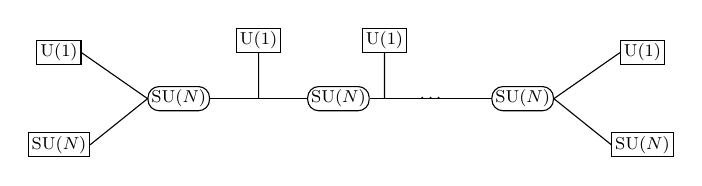
\begin{tikzpicture}[baseline=(G1.center),scale=0.78,transform shape,
  fl/.style={draw,rectangle,inner sep=1.6pt,font=\footnotesize},
  ga/.style={draw,rounded corners=4pt,inner sep=1.6pt,font=\footnotesize}]
  \node[ga] (G1) at (0,0) {$\mathrm{SU}(N)$};
  \node[ga] (G2) at (2.6,0) {$\mathrm{SU}(N)$};
  \node[ga] (G3) at (5.6,0) {$\mathrm{SU}(N)$};
  \node[font=\footnotesize] at (4.1,0) {$\cdots$};
  \node[fl] (UL) at (-1.95,0.75) {$\mathrm{U}(1)$};
  \node[fl] (SL) at (-1.95,-0.75){$\mathrm{SU}(N)$};
  \node[fl] (U12) at (1.3,0.95) {$\mathrm{U}(1)$};
  \node[fl] (U23) at (3.35,0.95) {$\mathrm{U}(1)$};
  \node[fl] (UR) at (7.55,0.75) {$\mathrm{U}(1)$};
  \node[fl] (SR) at (7.55,-0.75){$\mathrm{SU}(N)$};
  \draw (UL.east) -- (G1.west);
  \draw (SL.east) -- (G1.west);
  \draw (G1.east) -- (G2.west);
  \draw (U12.south) -- (1.3,0);
  \draw (U23.south) -- (3.35,0);
  \draw (G2.east) -- (G3.west);
  \draw (G3.east) -- (UR.west);
  \draw (G3.east) -- (SR.west);
\end{tikzpicture}
\end{gathered}
  \tag{4.26}
\end{equation}
其中我们在单穿刺点下面画了横线（于是只有 $0$ 与 $\infty$ 是满穿刺点）。

这个线性箭图规范理论描述对应于黎曼面的一个特定退化极限。我们要强调，其他极限会牵涉更复杂的 tinkertoy；除非每一块裤子都包含一个单穿刺点，它们通常没有拉氏量描述。正如习题 4.13 所得，无质量情形的 SW 曲线为
\begin{equation}
  x^N=\sum_{k=2}^{N}\frac{P^{(k)}_{n-4}(z)}
    {(z-z_1)\cdots(z-z_{n-2})\,z^{k-1}}\,x^{N-k},
  \tag{4.27}
\end{equation}
其中 $P^{(k)}_{n-4}$ 表示 $n-4$ 次多项式。

% [Tutor Note: p.42 式 (4.27) 的两处可核对结构：右边每一项分母含 $(z-z_1)\cdots(z-z_{n-2})$ 与 $z^{k-1}$，分子为 $n-4$ 次多项式------总极点阶数在 $z=0$ 处为 $k-1$、在有限穿刺点处为 1，与 (4.25)(4.24) 的极点阶数"满 $k-1$、单 $1$"一致；$N=2$ 时退化为二重覆盖 $\Sigma\to\mathbb{CP}^1$ 的定义方程。]

\begin{exercise}{4.14}
考虑如下退化极限：除某一个 $j$ 使 $z_{j+1}/z_j\to+\infty$ 之外，所有 $z_{i+1}/z_i$ 都保持不变（且 $|z_{i+1}/z_i|>1$）。验证曲线中 $x/z_j$ 保持有限的那一部分取 (4.27) 的形式，只是把 $n$ 换成 $j+2$ 并附加上质量项。特别地，新的穿刺点是满穿刺点。
\end{exercise}
